\documentclass[12pt]{article}
\usepackage[hmargin=2.0cm,vmargin=1cm]{geometry}
\usepackage[utf8]{inputenc}
\usepackage{graphicx}
\usepackage{float}
\usepackage{natbib}
\usepackage{amsmath}

\title{\begin{LARGE}
{HW2 ISM, Radiative transfer and processes}
\end{LARGE}}

\author{Juan Nicol\'as Garavito Camargo}

\begin{document}
\maketitle


\begin{LARGE}
\textbf{1.}
\end{LARGE}

If the source function can be approximated as: 

\begin{equation}\label{approx}
S(\tau) \approx S(\tau_{*}) + S'(\tau_*)(\tau - \tau_*) + \dfrac{1}{2}S''(\tau_*)(\tau-\tau_*)^2	
\end{equation}

Then the full general solution for the radiative transfer can be writen as:

\begin{equation}\label{sol}
I_{\nu}(\tau_1, \mu) = I_{\nu}(\tau_2, \mu) e^{-(\tau_2 - \tau_1)/\mu} + \dfrac{1}{\mu}\int_{\tau_1}^{\tau_2}S_{\nu}(\tau ')e^{-(\tau ' - \tau_1)/\mu} d\tau '
\end{equation}

\begin{equation}
I_{\nu}(\tau_1, \mu) = I_{\nu}(\tau_2, \mu) e^{-(\tau_2 - \tau_1)/\mu} + 
\dfrac{1}{\mu} \int_{\tau_1}^{\tau_2} e^{-(\tau ' - \tau_1)/\mu} d\tau ' 
\left[  S(\tau_{*}) + S'(\tau_*)(\tau ' - \tau_*) + \dfrac{1}{2}S''(\tau_*)(\tau '-\tau_*)^2 \right] d\tau '
\end{equation}

Now I treat the 3 integrals separately:\\

The first integral involving the term $S(\tau_*)$ is:

\begin{equation}\label{int1}
\int_{\tau_1}^{\tau_2}e^{-(\tau ' - \tau_1)/\mu} S(\tau_*) d\tau ' =
S(\tau_*)\int_{\tau_1}^{\tau_2}e^{-(\tau' - \tau_1)/\mu} d\tau ' = S(\tau_*) (-\mu) \left[ e^{-(\tau_2 - \tau_1)/\mu} - 1 \right]
\end{equation}

The second integral corresponding to the $S'(\tau_*)$ term:

\begin{equation*}
\int_{\tau_1}^{\tau_2}e^{-(\tau ' - \tau_1)/\mu} S'(\tau_*)(\tau ' - \tau_*) d\tau ' = S'(\tau_*) \int_{\tau_1}^{\tau_2}e^{-(\tau ' - \tau_1)/\mu} (\tau ' - \tau_*)
d\tau ' = -\mu S'(\tau_*)(\mu - \tau_* + \tau')e^{-(\tau ' - \tau_1)/\mu}
\end{equation*}

\begin{equation}\label{int2}
= -\mu S'(\tau_*)\left[ (\mu - \tau_* + \tau_2)e^{-(\tau_2 - \tau_1)/\mu} - (\mu - \tau_* + \tau_1) \right]
\end{equation}


Finally the third integral correspoding to the $S''(\tau_*)$ term is:

\begin{equation*}
\dfrac{1}{2}\int_{\tau_1}^{\tau_2}e^{-(\tau ' - \tau_1)/\mu} S''(\tau_*)(\tau ' - \tau_*)^2 d\tau' = \dfrac{S''(\tau_*)}{2} \int_{\tau_1}^{\tau_2}e^{-(\tau ' - \tau_1)/\mu} (\tau ' - \tau_*)^2 d\tau'  
\end{equation*}

\begin{equation*}
 =  \dfrac{S''(\tau_*)}{2} \left[-\mu (\tau_{*}^2 - 2\tau_*(\mu+\tau') + 2\mu^2 + 2\mu \tau' + \tau'^2)e^{-(\tau'-\tau_1)/{\mu}} \right]
\end{equation*}

\begin{equation}\label{int3}
= \dfrac{-\mu S''(\tau_*)}{2} \left[ (\tau_{*}^2 - 2\tau_*(\mu+\tau_2) + 2\mu^2 + 2\mu \tau_2 + \tau_{2}^2)e^{-(\tau_2 -\tau_1)/{\mu}} - (\tau_{*}^2 - 2\tau_*(\mu+\tau_1) + 2\mu^2 + 2\mu \tau_1+ \tau_{1}^2) \right]
\end{equation}

If $\tau_* = \mu$ and $\tau_1 = 0$ the terms that would be affected are Eq.\ref{int2} \& Eq.\ref{int3}
correspondly.

\begin{equation}
 = -\mu S'(\tau_*)\left[ \tau_2 e^{-(\tau_2-\tau_1)/\mu} - \tau_1\right] = -\mu S'(\tau_*) \tau_2 e^{-\tau_2/\mu} \approx 0
\end{equation}

\begin{equation}
= \dfrac{-\mu S''(\tau_*)}{2} \left[ (\mu^2 + \tau_{2}^2)e^{-(\tau_2 -\tau_1)/{\mu}} - (\mu^2 + \tau_{1}^2) \right] = \dfrac{-\mu S''(\tau_*)}{2} ( -\mu^2 ) = \dfrac{\mu^3 S''(\tau_*)}{2}
\end{equation}


\begin{LARGE}
\textbf{2.}
\end{LARGE}


\begin{equation}
I_{\nu} = I_{\nu}(0)e^{-\tau_{\nu}} + B_{\nu}(T)\left[ 1 - e^{-\tau_{\nu}} \right]
\end{equation}

When the source is observed trough the nebula:

\begin{equation}\label{I1}
I_{\nu, 1 } = I_{\nu}(T_s)e^{-\tau_{\nu}} + I_{\nu}(T_n)\left[ 1 - e^{-\tau_{\nu}} \right]
\end{equation}

\begin{equation}\label{I2}
I_{\nu, 2} = I_{\nu}(T_n)\left[ 1 - e^{-\tau_{\nu}} \right]
\end{equation}

Substracting Eq.\ref{I1} \& Eq.\ref{I2}

\begin{equation}
I_{\nu, 1} - I_{\nu, 2} = I_{\nu}(T_s)e^{-\tau_{\nu}}
\end{equation}



\begin{equation}
-\tau_{\nu} = Ln \left( \dfrac{I_{\nu, 1} - I_{\nu, 2}}{I_{\nu}(T_s)}  \right)
\end{equation}

\begin{LARGE}
\textbf{3.}
\end{LARGE}

\begin{figure}[H]
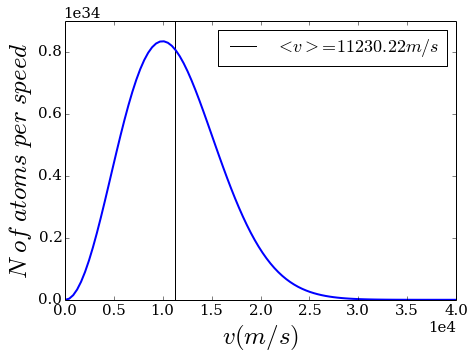
\includegraphics[scale=0.5]{mbv.png}
\caption{Velocity distribution for $10^{38}$Hydrogen atoms 
in the solar photosphere\label{mbv}}
\end{figure}

1. \\
Figure \ref{mbv} show the velocity distribution of thw $10^{38}$ atoms
in the solar photosphere. The black vertical line shows the typical
speed of a Hydrogen atom, which was computed as follows:

\begin{equation}
<v> = 2\int_0^{\infty} \left( \dfrac{m}{2\pi KT}  \right)^{3/2} 4\pi v^3 e^{-mv^2/KT}
\end{equation}

\begin{equation}
<v> = 8\pi \left( \dfrac{m}{2\pi KT}  \right)^{3/2} \left(\dfrac{KT}{m}\right)^4
= 2 \left( \dfrac{2}{\pi} \right)^{1/2} \left( \dfrac{KT}{m}  \right)^{1/2}
\end{equation}

\begin{equation}
<v> = 11203.22 m/s
\end{equation}

2. \\ 

The number of photons (N1) within a 1\% of $<v>$ can be computed with the CDF as follows:


\begin{equation}
N1 = erf(v/\sqrt{2}a) - \sqrt{\dfrac{2}{\pi}} \dfrac{v e^{-v^2/2a^2}}{a} \Bigg|_{0.99<v>}^{1.01<v>}  = 9.07\times 10^{35} 
\end{equation}

3. \\

The Doppler shifht due to the speed $<v>$ would be:

\begin{equation}
\dfrac{\nu}{\nu_0} = (1 + <v>/c) =  1.000037
\end{equation}

4. \\ 


\begin{LARGE}
\textbf{4.}
\end{LARGE}

To show that $h \nu << KT$ for HII regions we select the extreme case that
corresponds to $\lambda = 1mm$. Using the fact the typical temperature 
of a HII region is $10^4$K we found that: 

\begin{equation}
h \nu = 1.98 \times 10 ^{28} J
\end{equation} 

\begin{equation}
KT_{HII} = 1.38 \times 10^{-19} J
\end{equation}

Then for radio observations it is valid to work in the Rayleigh-Jeans limit.

\begin{equation}
B_{\nu}(T) = \dfrac{2\nu^2}{c^2}KT
\end{equation}

\begin{equation}
T_b = \dfrac{c^2}{2\nu^2K}I_{\nu}
\end{equation}

\begin{equation}
I_{\nu} = T_{\nu} (0)  e^{-\tau_{\nu}} + B_{\nu}(T)(1- e^{-\tau_{\nu}})
\end{equation}

\begin{equation}
\dfrac{2 \nu^2 K}{c^2} T_{\nu} = \dfrac{2 \nu K}{c^2}T_b(0)e^{-\tau_{\nu}} + \dfrac{2 \nu^2 K}{c^2} T(1 - e^{-\tau_{\nu}})
\end{equation}

\begin{equation}
T_{\nu} = T_b (0)  e^{-\tau_{\nu}} + T(1- e^{-\tau_{\nu}}) 
\end{equation}

\end{document}
